\section{Economía de Colombia}
Para la creación de un modelo de predicción de la TRM de Colombia, tomando como hipótesis de trabajo que existe un número finito y reducido de variables de aporte que regulan el valor de la misma a través de los ingresos por exportación y su contribución a la economía nacional, se debe primeramente comprender y definir estos conceptos. La sección del marco teórico que cubre la economía de Colombia, tiene como finalidad abarcar los siguientes temas. 

\begin{enumerate}
	\item Definir correctamente el concepto de tasa de cambio y su específico colombiano, la tasa de mercado representativa, desentrañando la formula que usa la Superintendencia Bancaria para su valuación diaria.
	\item Entender las bases del comercio internacional de Colombia y cuales son sus principales productos de exportación, sobre todo con el afán de identificar correctamente candidatos como variables de aporte para alimentar de datos el modelo de aprendizaje automatizado. 
	\item Por último, especificar el funcionamiento de los elementos financieros derivados de compra de divisas tales como los \emph{forward} y su correspondiente reglamentación bajo la leyes de Colombia. 
\end{enumerate}

Entender el funcionamiento de la economía de Colombia, sus principales componentes de exportación, y los marcos legales que rigen las estructuras de la TRM y los productos financieros de compra y venta de divisas, nos da luces no solo para entender correctamente el problema, sino para plantear propuestas de solución matemáticas que tengan una amplia correlación entre el modelo abstracto y el comportamiento en la vida real del proceso. 

\subsection{La Tasa de Cambio}
La moneda de un país tiene una equivalencia en moneda de otro y ese valor se conoce como tasa de cambio. Explicamos el concepto apoyados en los escritos del autor Mauricio Cárdenas \cite{cardenas}. También es importante explicar porqué los productos de exportación tienen un efecto en la canasta de divisas y la balanza de pagos \cite{crisisCambiarias}.   

\subsection{La TRM}
Dennis Robertson \cite{robertson} definió el dinero como \textit{"todo aquello generalmente aceptado para el pago de una obligación"}. El dinero en su forma más simple es el medio de pago de total liquidez, constituido por el \textit{efectivo} (billetes y monedas) y puesto en circulación por la Banca Central y por el \textit{dinero bancario}, correspondiente a los depósitos en bancos comerciales que son transferibles por medio de cheque. 

El intercambio de bienes y comercio internacional se realiza tomando como premisa que países con diferente moneda tendrán que llegar a algún tipo de mecanismo para compensar las compras, ventas y pagos de las mismas entre ambos actores. A falta de una moneda común (por lo menos en términos legales) el mecanismo que rige dicha condición de medio de operación es la tasa de cambio.

\subsubsection{Concepto: Tasa de Cambio}
Para entender el concepto de la tasa representativa de mercado, es importante primero entender el concepto de tasa de cambio. Dicha idea es muy sencilla, y gira entorno al valor de una moneda en relación con otra \cite{30seconds}. En épocas pasadas, el tipo de cambio era fijo, pero esta teoría ha quedado atrás con la implementación de tipos de cambio de flotación libre. La preocupación de los gobiernos gira en procurar mantener un determinado tipo de cambio ni estimule la revalorización de la moneda, ni mucho menos genere una devaluación de la misma \cite{cardenas}. 

\subsubsection{Devaluación de la Moneda} 
Se entiende como devaluación monetaria la pérdida del valor nominal de la moneda nacional frente a otra u otras monedas extranjeras. Las causas generadoras de la devaluación se pueden sintetizar principalmente en dos:

\begin{itemize}
	\item Falta o disminución de la demanda de la moneda nacional.
	\item Una mayor demanda de la moneda extranjera por parte de los consumidores y comerciantes de la nación.
\end{itemize}

En un sistema de cambio libre (dólar de flotación), en el cual la intervención del Banco de la República es nula, la devaluación toma el nombre de \textit{depreciación}. 

\subsubsection{Apreciación de la Moneda Local}
A veces, por causas externas a la economía de un país, la moneda local se ve sobrevaluada, sea por la abundancia de dólares procedentes del exterior o por el ingreso de capitales extranjeros al país. Esto genera que haya más reservas de dólares, provocando que la moneda local se aprecie por la mayor oferta de los capitales extranjeros. 

\subsubsection{Dólar de Flotación}
El 25 de septiembre de 1999, la Junta Directiva del Banco de la República de Colombia optó por desmontar la banda cambiaría y dar paso al dólar flotante. Cuando el precio de la divisa se mueve por libre juego de la oferta y la demanda, sin límite de techos o pisos, se habla de un régimen de flotación. La flotación implica que el Banco de la República no tendrá en adelante ninguna injerencia en la fijación del precio del dólar \cite{cardenas}. 

Las oportunidades en las cuales el estado ha tratado de varias formas de estabilizar la moneda y el tipo de cambio no han sido pocas. El país ha pasado a través de ciclos de revaluación y devaluación alternados, ambos con impactos negativos para la economía. 

\begin{enumerate}
	\item En el año 2007 el Gobierno Nacional intentó frenar el ingreso de dólares producto de capital golondrina con medidas de cautelas de depósitos de un cuarenta por ciento del valor durante seis meses, tratando de evitar la especulación (Decreto 2466 MINHACIENDA, Junio 2007)
	\item La disminución de los capitales y el aumento del desempleo llevó al Gobierno Nacional a desarticular dicha medida en el año 2008 (Decreto 1888 MINHACIENDA, Mayo 2008)
	\item En el año 2012 el Banco de la República tomo la estrategia de compras diarias de treinta millones de dólares como forma de mantener la moneda estable y lejos de la apreciación (Empresarios piden bajar tasas de interés por caída del dólar. (Enero 27 del 2012, Portafolio, pp.3)
	\item Hacia el año 2014 el Banco de la República, habiendo conseguido su meta de una tasa de cambio estable, redujo notablemente sus esfuerzos de compras de la divisa americana. Lamentablemente hacia mediados del 2015, la caida de los precios del petroleo tuvo un efecto nefasto en la devaluación del peso colombiano, que llegaría a tasas de cambio a finales del año cercanas a los \$3,300 pesos. 
\end{enumerate}

\subsubsection{La TRM (Tasa Representativa del Mercado)}
La Superintendencia Financiera de Colombia es la que calcula y certifica diariamente la TRM con base en las operaciones registradas el día hábil inmediatamente  anterior  y  la  define  de  la  siguiente  manera  (Circular  Reglamentaria Externa del Banco de la República DODM-146, 2015):

	\begin{quote}La  tasa  de  cambio  representativa  del  mercado  (TRM)  es  la  cantidad de pesos colombianos por un dólar de los Estados Unidos (antes del 27 de noviembre de 1991 la tasa de cambio del mercado colombiano estaba dada por el valor de un certificado de cambio). La TRM se calcula con base en las operaciones de compra y venta de divisas entre intermediarios financieros que transan en el mercado cambiario colombiano, con cumplimiento el mismo día cuando se realiza la negociación de las divisas.
	\end{quote}

La Superintendencia Financiera de Colombia no determina el valor de la TRM sino de un elemento derivado de las operaciones de compra y venta de la misma. Son los agentes de operación (exportadores que venden sus productos en dólares y los deben canjear a pesos colombianos e importadores que compran sus productos en dólares y para tal fin cambian sus pesos colombianos). Ambos obedecen a fuerzas del mercado que dan forma y materializan la valorización.

\subsection{Exportaciones de Colombia}
Si bien no buscamos ser expertos en ninguno de los tipos de exportación que hace Colombia, es importante en esta sección describir uno a uno los rubros con mayor contribución, ya que serán nuestras variables independientes para aplicar en el proceso de aprendizaje automatizado y modelar el comportamiento futuro de la TRM. 

\subsubsection{El Petróleo}
Del petróleo se dice que es el energético más importante en la historia de la humanidad, que es un recurso no renovable que aporta el mayor porcentaje del total de la energía que se consume en el mundo. En cuanto a Colombia, hace parte del grupo de países en el mundo que tiene petróleo, sin llegar a ser un país petrolero; su producción para el año 2015 tan solo alcanzó un millón de barriles diarios, de los cuales no todos son clasificados como los mejores, ya que no alcanzan según las normas API el nivel superior a 26 grados \cite{cardenas}. 

En Colombia los recursos naturales no renovables, entre ellos, los hidrocarburos, son propiedad del Estado. La política petrolera es definida por el Gobierno Nacional a través del Ministerio de Minas y Energía, y hasta el año 2003 Ecopetrol era la empresa encargada de su ejecución. 

\subsubsection{El Carbón}
Colombia, en cuanto a recursos carboníferos se refiere, ocupa dentro de los países latinoamericanos un lugar privilegiado, pues cuenta con las mayores reservas y cuenta con gran variedad de calidades. Este potencial carbonífero está distribuido en las tres cordilleras principales, correspondiendo la mayor parte a la cordillera oriental \cite{cardenas}. Colombia es el país con mayores reservas de carbón en América Latina, cuenta con recursos potenciales de 16,992 millones de toneladas (MT) de los cuales 7,063 MT son medidas, 4,571 MT son indicadas, 4,237 MT son inferidas y 1,119 MT son recursos hipotéticos. Por otra parte, es el sexto exportador de carbón del mundo, con una participación de 6,3\%, equivalente a 50 MT anuales de carbón \cite{carbonMain}. 

La importancia del carbón colombiano, más que por sus características, es por su posición estratégica (particularmente en las minas de la Guajira), pues facilita el acceso al mercado europeo y norteamericano, y porque ha logrado, con relativo éxito, la conquista de dichos mercados por su precio y calidad respecto al de los carbones procedentes de Australia e Indonesia \cite{cardenas}. Con la tasa de explotación actual, las reservas medidas de carbón en Colombia aseguran más de 120 años de producción, suficientes para participar a gran escala en el mercado internacional y abastecer la demanda interna \cite{carbonMain}

El carbón, fuente generadora de divisas y de empleo, concentra el 47\% de la actividad minera nacional y representa el 1\% del producto interno bruto colombiano con algo más de 3,4 billones de pesos \cite{carbonMain}. En los últimos años se ha consolidado en el segundo producto de exportación nacional  después del petróleo y se estima que bajo las condiciones de mercado actuales, entre el 2010 y 2015 podría superar las exportaciones de petróleo.

\subsubsection{El Café}
El café es uno de los productos básicos del mundo que más se comercializa. Es el principal producto agrícola de Colombia, y de él depende un porcentaje significativo de la economía y el sustento de gran parte de la población. El café Colombiano es reconocido a nivel mundial a través de su marca registrada Juan Valdez. Dado que es una de las exportaciones que continua creciendo, es de esperar que sea una fuente de divisas y exista una correlación estrecha entre el precio del café y el valor de la TRM. 

Se cree que los Jesuitas fueron los primeros en cultivar café en Colombia en la región del Orinoco, hacia 1732. Posteriormente, difundieron su cultivo por el sur del país. El párroco de Sálazar de las Palmas, Francisco Romero, ferviente admirador de la planta, impuso como penitencia a sus feligreses la siembra de cafetos según la gravedad de los pecados. Su ejemplo, seguido por otros sacerdotes y así se propagó el café por el nororiente del país. A mediados del siglo XIX el cultivo del café se expandió del norte al centro y occidente del territorio. A finales de ese siglo, se consolidó como cultivo de exportación. Desde cuando comenzaron a tener forma ordenada el cultivo y la actividad exportadora de café en Colombia, el producto ha estado estrechamente ligado al desarrollo y bienestar del país \cite{cafeMain}.

Actualmente, el café genera más de 1 millón de empleos permanentes de los cuales 800,000 se ocupan de las labores agrícolas. Más de 500,000 familias se benefician de su cultivo. Todos los cafetales sembrados hasta 1993 estaban en producción y las exportaciones ascendieron a cerca de 532,000 sacos. Para mediados de la década de los 90, el café representaba mucho más de la mitad del valor total de las exportaciones colombianas, y en los años pico de 1995 y 1996 el café significó cerca del 70 por ciento del valor total delas exportaciones. Alrededor de 1 millón de hectáreas están sembradas en café, lo que equivale al uno por ciento del área total de Colombia. Las zonas cafeteras se distribuyen a lo largo de las pendientes de las cordilleras en un microambiente especial de clima templado. La mayor cantidad de cultivos se encuentra en los departamentos de Antioquia, Caldas, Risaralda, Quindío, Tolima y Valle del Cauca \cite{cafeMain}

Colombia tiene, pues, gran tradición como país productor y exportador de café. La actividad cafetera favoreció el aumento y la expansión de la industria manufacturera, el crecimiento de las ciudades, el desarrollo de la infraestructura de transporte, la formación del sector financiero y la vinculación del país al comercio internacional.

\subsubsection{El Níquel}
El  desarrollo  de  la  minería  en  Colombia, aún en proceso de mejoramiento, muestra el adelanto de la industria del Níquel como una de las que mayores beneficios le han dado  al  país,  al  lado  de  los  grandes  progresos que se tienen en el sector carbonífero, siendo estas por excelencia las exportaciones tradicionales del país, en lo que compete al sector minero, con el petróleo y carbón \cite{niquelMain}.

La importancia del níquel radica en las aleaciones con otros elementos para dar fuerza y resistencia a la corrosión en amplias variaciones de temperatura. Se utiliza principalmente en aleaciones con el hierro y el acero para las fabricaciones de aceros inoxidables empleados en la industria en forma general. En Colombia, los recursos identificados pertenecen al grupo de las lateritas niquelíferas, producto de la alteración de las rocas ultramáficas del conocido sistema tectónico ofiolítico \cite{cardenas}.

En Colombia existen seis yacimientos de Níquel, tres de ellos están localizados en la región Caribe, en el departamento de Córdoba (Cerro Matoso, Planeta Rica  y Uré). Los tres restantes se encuentran en el departamento de Antioquia (Ituango, Morro Pelón y Medellín) \cite{niquelMain}.

Cerro Matoso es una mina de extracción de Níquel integrada con el proceso de  fundición, que además combina los depósitos lateríticos de Níquel más ricos del mundo, con una fundición de Ferroníquel a bajo costo, lo cual la ha convertido en uno de los productores de Ferroníquel con más bajo costo de producción en el mundo \cite{niquelMain}.

Colombia es el primer productor de Níquel en Suramérica y el tercero en Centroamérica y el Caribe, después de Cuba y República Dominicana. Cerro Matoso aporta el 10\% de la producción mundial de Ferroníquel y un 3\% de la producción mundial de Níquel. La producción industrial se hace en lingotes de Ferroníquel con un contenido de 37,5\% de Níquel \cite{niquelMain}.

\subsubsection{El Oro}
De acuerdo a la Contraloría General de la República,se afirma que en Colombia hay 17 departamentos y 80 municipios donde se llevan a cabo procesos de extracción artesanal, pequeña o industrial de oro y según la UPME, Antioquía y   Bolívar poseen la mayor cantidad de minas del país y producen alrededor de  18.8  MT de oro anuales, si bien departamentos como Chocó, Córdoba, Caldas y Tolima  también tienen amplia presencia de la actividad extractiva del metal \cite{oroMain}.

La actividad de extracción del oro en el país se podría nominar como atomizada, es decir, existen múltiples actividades de extracción en diferentes zonas, la mayoría de las cuales no cuenta con una legalidad o formalización en su actividad. Tomando datos oficiales, existen 4,133 unidades de minería que son  equivalentes al 29\% de la minería con o sin título minero, de las cuales 3,584 son ilegales. Esto representa el 40\% del total de la ilegalidad de minería en el país, lo cual indica que de cada cinco unidades ilegales dos pertenecen al oro \cite{oroMain}. 

Lamentablemente la explotación del oro tiene una connotación negativa en el país. La Dra. Adriana Arango nos ilustra \cite{arango_2017}:

\begin{quote}
Después de la independencia de Colombia, el oro pasó a ser propiedad de la Nación y desde entonces la minería se convirtió en un sector económico regulado por la legislación nacional. Luego de muchos años de explotación, mayormente por la industria, medianos y pequeños mineros, los grupos armados pasaron a tomar parte en el negocio de la minería de oro, ya sea extorsionando mineros y/o extrayendo oro de forma ilegal. Esto ocurrió a partir de las negociaciones formales de paz entre el gobierno y la guerrilla en 2012, donde el oro se convirtió en una actividad económica que sostenía las organizaciones armadas. A pesar de que los grupos insurgentes (FARC y ELN) estaban adquiriendo un promedio de \$600 millones al año, proveniente del negocio de cultivos ilícitos, extorsión, secuestro, ganado robado, y otras fuentes; el oro también se volvió lucrativo debido a su pequeño volumen y su alto valor. El incremento de explotación de oro por parte de grupos armados incrementó con el aumento en el control de cultivos ilícitos en el país. Así, la extracción de oro pasó de 47.8 MT en 2009 a 66.2 MT en 2012, cifra que se ha mantenido hasta el 2016.
\end{quote}

Es interesante que los ingresos por la extracción del oro pasan en gran parte por la economía informal. ¿Cuál es el impacto de ingresos informales del oro en la tasa de cambio del dólar en Colombia? Si bien esta no es una pregunta que nos hacemos en el proyecto de investigación, se podrá contestar cuando se mida el coeficiente de determinación y el coeficiente de correlación de Pearson en el capítulo 4 de análisis y discusión de resultados.  

\subsubsection{El Banano}
El banano es el cultivo que ocupa el primer lugar en las exportaciones agropecuarias menores. Las principales zonas de cultivo son las de Urabá (72\% de la producción) y Santa Marta. Los principales problemas en el cultivo son las plagas, los problemas socio laborales, los vientos huracanados y problemas internacionales por la aparición de otros tipos de banano de mejor aceptación. Aunque el volumen de producción de Colombia se ve superado por Ecuador, existen óptimas condiciones para la producción a bajos costos. La fruta es cultivada desde el nivel del mar hasta alturas de 2,200 metros. El consumo nacional ha mejorado y cada vez se han ido extendiendo los cultivos en algunas fincas del Quindío y del Valle del Cauca, intercalando con el plátano \cite{bananoC}.

Colombia ha tenido una relativa larga tradición como productora y exportadora neta de banano de exportación tipo \emph{Cavendish Valery}. La agroindustria bananera se ha desarrollado como una cadena agroexportadora tradicional, generando importantes divisas para el país, manteniendo su posición como exportadora neta, después del café y las flores. En el país existen dos tipos de banano: el banano de exportación y el banano criollo o de consumo interno \cite{bananoFINAGRO}.

\begin{itemize}
\item El banano de exportación: las regiones del Golfo de Urabá y el nororiente del departamento del Magdalena, se han especializado en la producción y exportación de banano y plátano con altos niveles de productividad e integración de los productores y comercializadores, gracias a las ventajas comparativas de localización y calidad de los suelos con respecto a otras zonas productoras del mundo.
\item El Banano Criollo: El banano criollo (común y murrapo) o de consumo interno, según datos del Ministerio de Agricultura, se produce principalmente en el Valle del Cauca, Tolima y Antioquia y tiene un área cosechada y una producción significativamente menores al de exportación.
\end{itemize}

La Asociación De Bananeros De Colombia \emph{AUGURA} es una corporación de derecho civil de interés colectivo, estrictamente gremial, que agrupa a los productores y comercializadoras internacionales de banano de Antioquia y Magdalena, zonas colombianas productoras de la fruta para los mercados internacionales. AUGURA como gremio busca asegurar que las exportaciones de banano se consoliden en los mercados internacionales, como resultados de procesos de producción sostenible que garanticen la conservación del recurso humano y natural, una justa distribución del ingreso y el bienestar social de los trabajadores de la industria y de los habitantes de las zonas de producción \cite{bananoAUGURA}.

\subsubsection{Las Rosas}
Las primeras noticias que se tienen en Colombia de la producción de flores con  fines comerciales, es de los primeros años de la década del 30 cuando algunos miembros de la sociedad bogotana, entre ellos granjeros de origen europeo, cultivaron jardines en los solares de las casas, crearon viveros y con ellos  los clubes de jardinería. Igualmente por esa época se realizaron las primeras  ferias de flores como la Exposición Mundial de Orquídeas en Medellín, primer antecedente de la Feria de las Flores actual \cite{cardenasRodriguez}.

Según Cárdenas y Rodríguez \cite{cardenasRodriguez}, el origen del comercio de flores en Colombia sin embargo fue la visión de un ciudadano norteamericano. 

\begin{quote}
Simultáneamente con los estudios de Cheever y otros estudiantes de las Universidades de Chicago y California, Edgar Wells Castillo un colombiano que residía en Estados unidos vio en la industria de las flores un excelente negocio ya que las condiciones climáticas de Colombia eran mejores que la tierra  y  el  clima de Estados Unidos. Allí conoció los pormenores de la industria y regreso al país con la ilusión de convertir a Colombia en uno de los principales países productores de flores. Wells junto con otros empresarios iniciaron la aventura de producir flor de corte, inicialmente para abastecer el mercado local pero el gran sueño era exportar a los Estados Unidos. Wells creo una de las primeras empresas de flores del país “Flores  Colombianas  Ltda.” la cual producía claveles y crisantemos y en octubre de 1965 enviaron el primer embarque a los Estados Unidos.
\end{quote}

La industria de las flores de corte en Colombia se inició con el cultivo del clavel, pompones, crisantemos y rosas. Posteriormente finalizando la década del  70 los cultivos se diversificaron. Con la evolución de los mercados, Colombia  tuvo que implementar políticas de diversificación de cultivos para seguir siendo  competitivos.  En  la  actualidad  se  exportan  más  de  50  tipos  de  flor  y  follajes,  lo  que  le  ha  permitido  al  país  seguir  ocupando el segundo lugar de exportaciones en el mundo. Igualmente  las  regiones  se  han  venido  especializando  en  los  cultivos, la Sabana de Bogotá produce rosas, claveles y alstroemerias, Antioquia crisantemos y follajes y Valle y el Eje Cafetero  follajes, helechos y flores tropicales. En la actualidad se producen y  exportan  principalmente rosas 30\%, clavel estándar 13\%, mini clavel 6\%, crisantemos 2\%, pompones 6\%, y otros tipos de flores 33\% \cite{cardenasRodriguez}

\subsubsection{Gasoleo}
El petrodiesel es el gasóleo extraído del petróleo. Se diferencia del biodiésel, que es el gasóleo extraído del aceite vegetal. En España se denomina gasóleo al combustible y diésel al motor diésel, aunque en América Latina es más común usar diésel para ambos, en Colombia se lo denomina ACPM, que son las siglas de Aceite Combustible Para Motores. Es una mezcla de hidrocarburos que se obtiene por destilación fraccionada del petróleo entre 250C y 350C a presión atmosférica. El gasóleo es más sencillo de refinar que la gasolina y suele costar menos. Por el contrario, tiene mayores cantidades de compuestos minerales y de azufre.

\subsection{Compendio de Exportaciones Colombia 2010 al 2016}
En la siguiente tabla figura el compendio de las principales exportaciones de Colombia, entre los años 2010 y 2016, que se utilizaron en el estudio para definir los principales regresores a entrenar con el modelo de aprendizaje automatizado. \\

\begin{figure}[H]
\centering
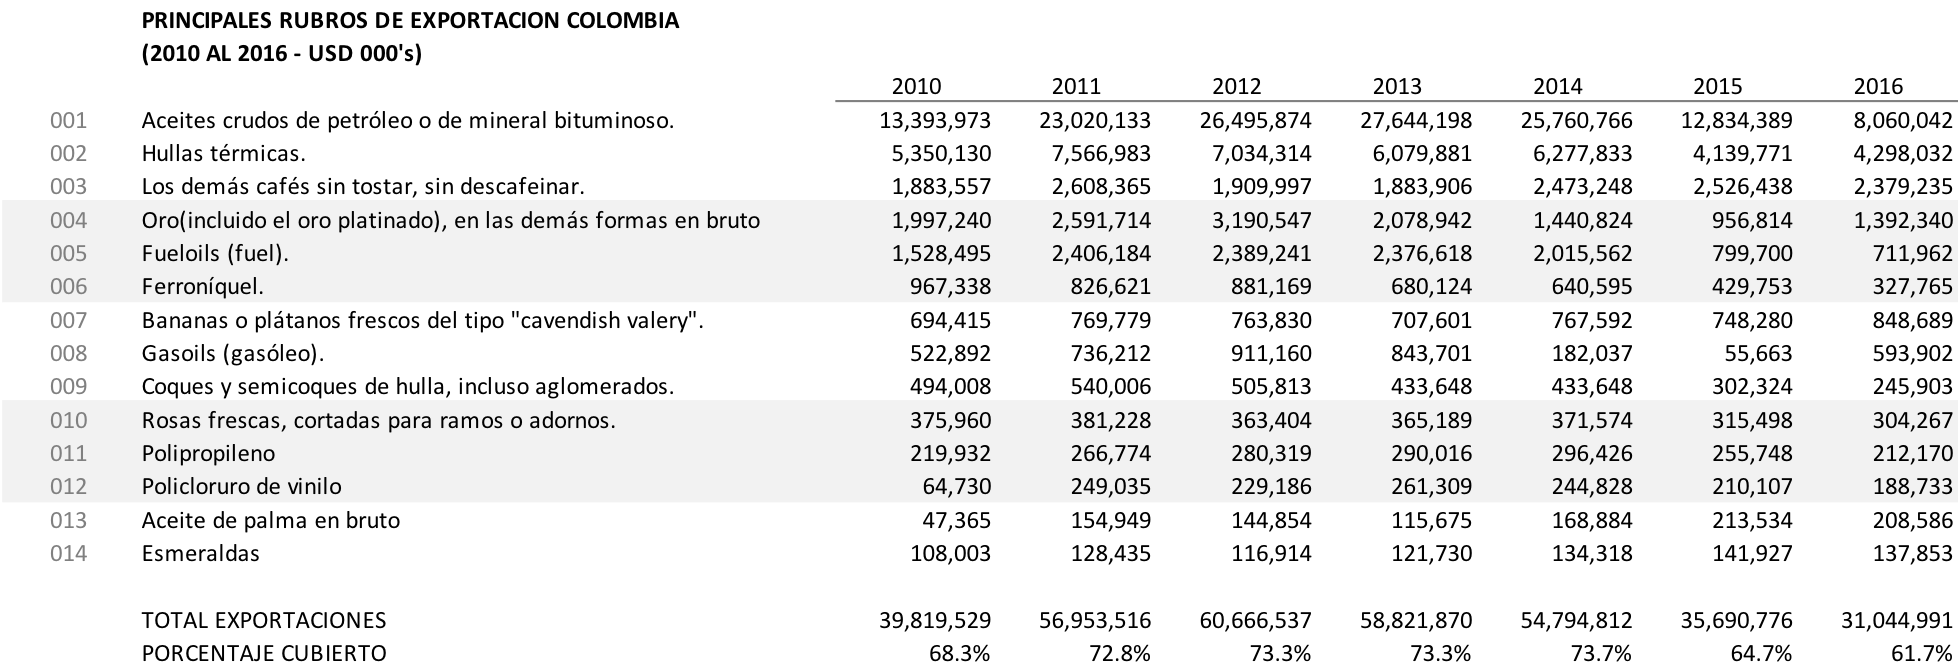
\includegraphics[width = 15cm]{ExportacionesColombia.png}
\caption{Principales Rubros de Exportación Colombia 2010-2016}
\end{figure}
